% !TeX spellcheck = cs_CZ

\documentclass[a4paper]{article}
\usepackage[english]{babel}
\usepackage[utf8x]{inputenc}
\usepackage[T1]{fontenc}
\usepackage{listings}
\usepackage[a4paper,margin=2cm]{geometry}
\usepackage{amsmath}
\usepackage{graphicx}
\usepackage[colorlinks=true, allcolors=blue]{hyperref}
\usepackage{wasysym} % smileys
\usepackage{fancyhdr}
\usepackage{tikz}
\setlength\parindent{0pt} % indent

% my commands:
\newcommand{\n}{\newline}
\newcommand{\tab}{\hspace{1cm}}

\begin{document}

\thispagestyle{fancy} % beware the difference between \thispagestyle and \pagestyle
\lhead{4th homework, 29-10-2019}
\rhead{Vilém Zouhar}

\section{Tetrahedron}

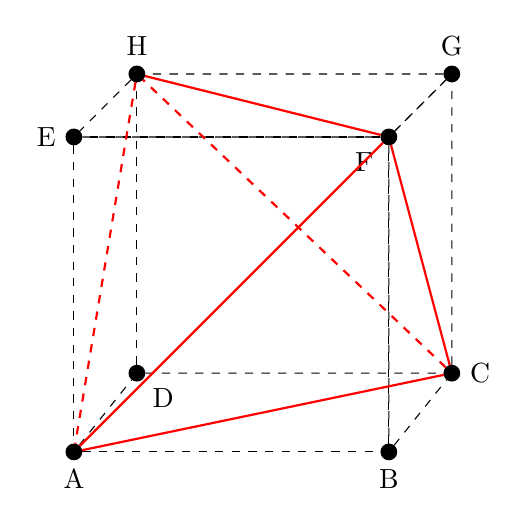
\begin{tikzpicture}
\foreach \n/\x/\l/\p in{
1/{( 0  , 0)}/{A}/below,
2/{( 4, 0)}/{B}/below,
3/{( .8, 1)}/{D}/south east,
4/{( 4.8, 1)}/{C}/right,
5/{( 0, 4)}/{E}/left,
6/{( 4, 4)}/{F}/south west,
7/{( 0.8, 4.8)}/{H}/above,
8/{( 4.8, 4.8)}/{G}/above
}
{
        \node[inner sep=2pt,circle,draw,fill,label={\p:\l}] (\n) at \x {};
    }
\draw[dashed] (1) -- (2) -- (6) -- (5) -- (1);
\draw[dashed] (5) -- (6) -- (8) -- (7) -- (5);
\draw[dashed] (2) -- (4) -- (8) -- (6) -- (2);
\draw[dashed] (1) -- (3) -- (4);
\draw[dashed] (3) -- (7);
\draw[thick, red,dashed] (4) -- (7) -- (1);
\draw[thick, red] (1) -- (4) -- (6) -- (7) -- (6) -- (1);
\end{tikzpicture}

\begin{tabular}{ | l | p{8cm} | l | l |}
    \hline
    type & description & example & \# \\
    \hline
    (4, 0, 0, 0) & id & (A)(C)(F)(H) & 1 \\
    \hline
    (1, 0, 1, 0) & rotation $2\pi/3$ around an axis between a point and the altitude to the opposing triangle & (A)(CFH) & 3 \\
    \hline
    \hline
\end{tabular}


\end{document}
